%прозрачки
\documentclass[trans]{beamer}
\usepackage[orientation=portrait,size=A4]{beamerposter}
%\usepackage[size=A4]{beamerposter}
\usepackage[utf8]{inputenc}
\usepackage[russian]{babel}

\DeclareMathOperator{\sn}{sn}
\DeclareMathOperator{\cn}{cn}
\DeclareMathOperator{\dn}{dn}
\DeclareMathOperator{\fu}{f}

\author{Павел Щелоковский}
\title{Термодинамический анализ несоразмерной фазы в одноосных собственных сегнетоэлектриках}
\date{2000}

%Tr2 = fig1a
%Tr3-1 = fig1b
%Tr3-2 = fig1c
%Tr4-1,2,3 = fig3a,b,c
%Tr5-1 = fig6
%Tr5-2 = fig5
%Tr6-1 = fig7
%Tr6-2 = fig8
%Tr7-1 = fig9

\begin{document}

\begin{frame}
\begin{equation*}
\mathrm{TP} - \mathrm{TP}_0 = 
 	                      \int^L_0 \left\{\frac{\sigma}{4} \left( \phi'' \right)^2 + 
 	                      \frac{\lambda}{2}\left(\phi\phi'\right)^2 + 
 	                      \frac{\delta}{2}\left(\phi'\right)^2 +
 	                      \frac{\alpha}{2}\phi^2 + \frac{\beta}{4}\phi^4 + 
 	                      \frac{\gamma}{6}\phi^6
 	                      \right\} dX	
\end{equation*}

\begin{equation*}
\Phi = \frac{\Phi_0}{L} \int_0^L \left[
            \left(\varphi''\right)^2 - g\left(\varphi\varphi'\right)^2 -
            \gamma\left(\varphi'\right)^2 +
            q\varphi^2 + \frac{p}{2}\varphi^4 + \frac{h}{3}\varphi^6
            \right] dX, \quad 
h = \gamma = 1
\end{equation*}

\begin{equation*}
\varphi^{(IV)} + 
g\left(\varphi^2\varphi'' + \varphi\left(\varphi'\right)^2\right) +
\gamma\varphi'' + q\varphi + p\varphi^3 + h\varphi^5 = 0
\end{equation*}

\begin{equation*}
\left(\varphi'\right)^2 = \sum_{n=0}^{\infty} a_n\varphi^{2n} \quad \rightarrow \quad
\left(\varphi'\right)^2 = \sum_{n=0}^N a_n\varphi^{2n}
\end{equation*}

\begin{equation*}
\varphi(x) = \frac{A\fu(bx, k)}{\sqrt{C - \fu^2(bx, k)}},
\end{equation*}

\begin{equation*}
\fu(bx, k) \in \{\sn(bx, k), \cn(bx, k), \dn(bx, k)\}
\end{equation*}

\begin{equation*}
\varphi^2(x) = Q
\frac{1-\frac{\cn(\omega x, k)}{\dn(\omega x, k)}}
{\frac{m_1}{n_1} -\frac{\cn(\omega x, k)}{\dn(\omega x, k)}}
\end{equation*}

\end{frame}

\begin{frame}
\begin{equation*}
\varphi(x) = a \cdot \sin(bx)
\end{equation*}

\begin{equation*}
\varphi(x) = a  \cdot \sn(bx, k)
\end{equation*}

\begin{equation*}
\begin{aligned}
\mathrm{TP} - \mathrm{TP}_0 =
                      \int^L_0 \left\{\frac{\sigma}{4} \left( \phi'' \right)^2 +
                      \frac{\lambda}{2}\left(\phi\phi'\right)^2 +
                      \frac{\delta}{2}\left(\phi'\right)^2 +\right.\\
                      \left.\frac{\alpha}{2}\phi^2 + \frac{\beta}{4}\phi^4 +
                      \frac{\gamma}{6}\phi^6
                      \right\}\;dX.
\end{aligned}
\end{equation*}

\center

\begin{figure*}
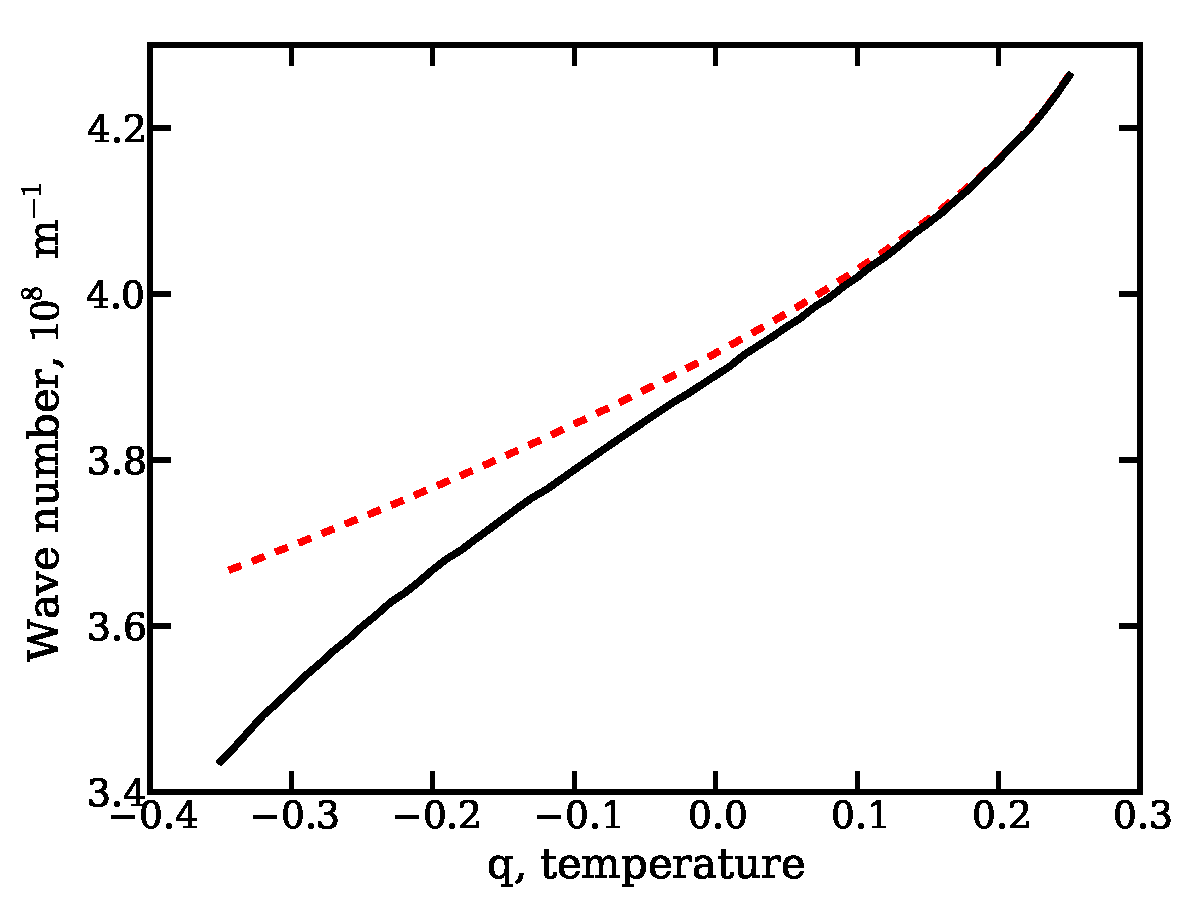
\includegraphics{figs/gpinit-wn.pdf}
\caption{$g$ и $p$ -- initial}
\end{figure*}

\end{frame}
\end{document}
